\documentclass[article]{jss}
\usepackage{algorithmic}
\usepackage{algorithm} 


%%\VignetteIndexEntry{Causal Inference: The pcalg R package}
%%\VignetteDepends{}


%           ^^^^^^^^^^^^^^^^ preserve comments (and all) in R chunks

%%%%%%%%%%%%%%%%%%%%%%%%%%%%%%
%% declarations for jss.cls %%%%%%%%%%%%%%%%%%%%%%%%%%%%%%%%%%%%%%%%%%
%%%%%%%%%%%%%%%%%%%%%%%%%%%%%%

%% almost as usual
\author{Markus Kalisch\\ETH Z\"urich \And
        Martin M\"achler\\ETH Z\"urich \And
      Diego Colombo\\ETH Z\"urich \And
    Marloes H. Maathuis\\ETH Z\"urich \And
  Peter B\"uhlmann\\ETH Z\"urich}
\title{Causal Inference using Graphical Models with the Package \pkg{pcalg}}

%% for pretty printing and a nice hypersummary also set:
\Plainauthor{Markus Kalisch, Martin M\"achler, Diego Colombo, Marloes
  H. Maathuis, Peter B\"uhlmann} %% comma-separated
\Plaintitle{Causal Inference using Graphical Models: The package pcalg} %% without formatting
\Shorttitle{Causal Inference} %% a short title (if necessary)

%% an abstract and keywords
\Abstract{
  The abstract of the article.
}
\Keywords{keywords, comma-separated, not capitalized, \proglang{R}}
\Plainkeywords{keywords, comma-separated, not capitalized, R} %% without formatting
%% at least one keyword must be supplied

%% publication information
%% NOTE: Typically, this can be left commented and will be filled out by the technical editor
%% \Volume{13}
%% \Issue{9}
%% \Month{September}
%% \Year{2004}
%% \Submitdate{2004-09-29}
%% \Acceptdate{2004-09-29}

%% The address of (at least) one author should be given
%% in the following format:
\Address{
  Markus Kalisch\\
  Seminar f\"ur Statistik\\
  ETH Z\"urich\\
  8092 Z\"urich, Switzerland\\
  E-mail: \email{kalisch@stat.math.ethz.ch}\\
  %% URL: \url{http://stat.ethz.ch/people/kalisch}
}
%% It is also possible to add a telephone and fax number
%% before the e-mail in the following format:
%% Telephone: +43/1/31336-5053
%% Fax: +43/1/31336-734

%% for those who use Sweave please include the following line (with % symbols):
%% need no \usepackage{Sweave.sty}

%% end of declarations %%%%%%%%%%%%%%%%%%%%%%%%%%%%%%%%%%%%%%%%%%%%%%%


\begin{document}


%% include your article here, just as usual
%% Note that you should use the \pkg{}, \proglang{} and \code{} commands.

\section{Introduction}
THIS DOCUMENTATION IS STILL UNDER CONSTRUCTION! \\

Understanding cause-effect relationships between variables is of primary
interest in many fields of science. Usually, experimental intervention is
used to find these relationships. In many settings, however, experiments
are infeasible because of time, cost or ethical constraints.

Recently, we proposed and mathematically justified a statistical
method (IDA) to obtain bounds on total causal effects based solely on
observational data [ANNALS]. Futhermore, we presented an experimental
validation of our method on a large-scale biological system [NATURE METHODS].

For further validation and broader use of this method, well documented and
easy to use software is indispensible. Therefore, we wrote the R package
\pkg{pcalg}, which incorporates the above mentioned method (IDA).

The objective of this paper is to introduce the R package \pkg{pcalg} and
explain the main range of functions.

To get started quickly, we show how two of the main functions can be used
in a typical application. Suppose we have a system described by some of variables
and many observations of this system. Furthermore, assume that it seems plausible that
there are no hidden variables and no feedback loops in the underlying
causal system. We are interested in the change of variable Y if we changed
the variable X by intervention, i.e., we seek the causal effect of X on Y.
To fix ideas, we have simulated an example data set with $p = 8$ continuous
variables with gaussian noise and $n = 5000$ observations, which we will
now analyse. First, we load the package \pkg{pcalg} and the data set.

\begin{Schunk}
\begin{Sinput}
>  library(pcalg)
>  ## load data matrix "dat"
>  data(gaussianData)
\end{Sinput}
\end{Schunk}

In the next step, we use the function \code{pc} to produce an estimate of
the underlying causal structure. Since this function is based on
conditional independence tests, we need to define two things: First, a
function that can compute conditional independence tests in a way that is
suitable for the data at hand. For standard data types (gaussian, discrete
and binary) we provide predefined functions. See the example section in the
help file of \code{pc} for more details. Secondly, we need a summary of the
data (sufficient statistic) on which the conditional independence function
can work. Each conditional independence test can be performed at a certain
significance level \texttt{alpha}. This can be treated as a tuning
parameter.

\begin{Schunk}
\begin{Sinput}
> ## use predefined test for conditional independence tests on gaussian data
> indepTest <- gaussCItest 
> ## the function gaussCItest needs as input the correlation matrix C and 
> ## the sample size n (see ?gaussCItest)
> suffStat <- list(C = cor(dat), n = 5000)
> ## estimate the causal structure
> pc.fit <- pc(suffStat, indepTest, p = 8, alpha = 0.01)
> ## plot the resulting causal structure
> plot(pc.fit, main = "")
\end{Sinput}
\end{Schunk}

\begin{figure}
  \begin{center}
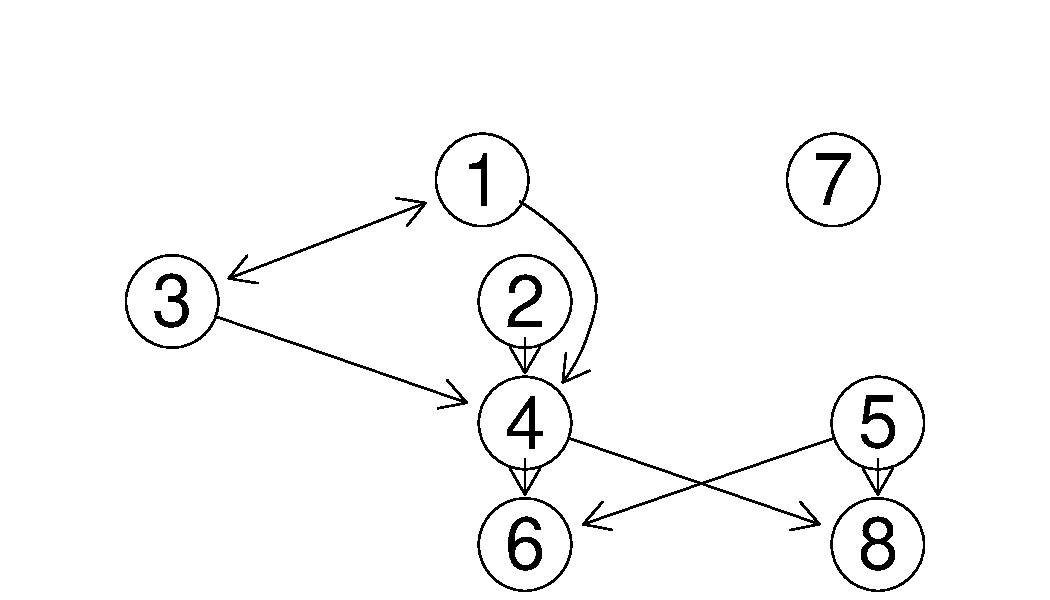
\includegraphics{pcalgDoc-exIntroPlot}
\caption{Estimated causal structure}
\label{fig:intro1}
\end{center}
\end{figure}

As can be seen in Fig. \ref{fig:intro1}, there are directed and bidirected
edges in the estimated causal structure. The directed edges show the
presence and direction of direct causal effects. The direction of the
bidirected edges, however, could not be decided by our method. Thus, they
represent some uncertainty in the resulting model. A fundamental property
of our method is, that some uncertainty of this kind sometimes remains,
even if an infinite amount of data is available.

Based on the inferred causal structure, we can estimate the causal
effect of an intervention. Suppose, we would increase variable $V1$ by
one unit, how much would variable 6 increase? Since the causal structure
was not identified perfectly, we cannot expect to get a unique
number. Instead, we will get a set of possible causal effects. This set can
be computed by using the function \code{ida}. To provide full quantitative
information, we need to pass the covariance matrix in addition to the
estimated causal structure.

\begin{Schunk}
\begin{Sinput}
> ida(1, 6, cov(dat), pc.fit@graph)
\end{Sinput}
\begin{Soutput}
[1] 0.3037948 0.2081007
\end{Soutput}
\end{Schunk}

Since we simulated the data, we know that the true value of the causal
effect is 0.296. Thus, one of the two estimates is indeed close to the true
value. Since both values are larger than zero, we can conclude, that
variable $V1$ has a positive causal effect on variable $V6$ (note that we have no
p-value to control the sampling error).

If we would like to know the effect of a unit increase in variable $V1$ on
variables $V3$, $V5$ and $V6$, we could simply call \code{ida} three
times. However, a faster way is to call the function \code{idaFast}, which
was taylored for such situations. Each row shows the set of effects on the
target variable indicated by the row names.

\begin{Schunk}
\begin{Sinput}
> idaFast(1, c(3,5,6), cov(dat), pc.fit@graph)
\end{Sinput}
\begin{Soutput}
    beta.tmp   beta.tmp
3 0.45481080 0.00000000
5 0.01623214 0.01927009
6 0.30379485 0.20810068
\end{Soutput}
\end{Schunk}

The true values for the causal effects are 0.441, 0, 0.296 for variables
$V3$, $V5$ and $V6$, respectively. The first row of the output,
corresponding to variable $V3$, is uninformative: Although one entry comes
close to the true value, the other estimate is 0. Thus, we cannot be sure
if there is a causal effect at all. The second row, corresponding to
variable $V5$, quite accurately indicates a causal effect that is very close
to zero or no effect at all. The third row, corresponding to variable $V6$,
was already discussed in the previous section on \code{ida}.

\section{Methodological background}
Our proposed method consists of two major steps. In the first step, the
causal structure is estimated. This is done by estimating a graphical
model. A graphical model is a map of the dependence structure of the data
and can thus be an interesting object by itself. In the second step, we use
the estimated causal structure and the do-calculus [PEARL] to calculate
bounds on causal effects.

\subsection{Estimating graphical models} \label{sec:gm} 
Graphical models
can be thought of as maps of dependence structures of a given probability
distribution or a sample thereof (see for example \cite{lauritzen}). In
order to illustrate the analogy, let us consider a road map. In order to be
able to use a road map, one needs two given factors. Firstly, one needs the
physical map with symbols such as dots and lines. Secondly, one needs a
rule for interpreting the symbols. For instance, a railroad map and a map
for electric circuits might look very much alike, but their interpretation
differs a lot. In the same sense, a graphical model is a map. Firstly, a
graphical model consists of a graph with dots, lines and potentially edge
marks like arrowheads or circles. Secondly, a graphical model always comes
with a rule for interpreting this graph. In general, nodes in the graph
represent (random) variables and edges represent some kind of dependence.

\subsubsection{Without hidden and selection variables}
An example of a graphical model is the Directed Acyclic Graph (DAG)
model. The physical map here is a graph consisting of nodes and arrows
(only one arrowhead per line) connecting the nodes. As a further
restriction, the arrows must be directed in a way, so that it is not
possible to trace a circle when following the arrowheads. The
interpretation rule is called d-separation. This rule is a bit more
intricate and we refer the reader to \cite{lauritzen} for more details
[ODER HIER ERKLAEREN?]. The interpretation rule can be used in the
following way when given a DAG model (FAITHFULNESS ERKLAEREN?): Two nodes
$X$ and $Y$ are d-separated by a set of nodes $S$, if and only if the
corresponding random variables $X$ and $Y$ are conditionally independent
given the set of random variables $S$.

Since the DAG model encodes conditional idependences, it seems plausible
that information on the latter helps to infer aspects of the former. This
intuition is made precise in the PC algorithm (CITE; PC stands for the
initials of its inventor Peter Spirtes and Clark Glymour) which was proven
to reconstruct the structure of the underlying DAG model given a
conditional independence oracle up to some ambiguity (equivalence class)
to be discussed below. In practice, the conditional independence oracle is
replaced by a statistical test for conditional independence. For situations
without hidden variables and under some further conditions it has been
shown that the PC algorithm using statistical tests instead of an
independence oracle is computationally feasible and consistent even for very
high-dimensional, sparse DAGs [PCpaper]. 

It is possible, that several DAGs encode the same list of conditional
independencies. However, one can show that these DAGs must share certain
properties. To be more precise, we have to define a colliding v-structure
as the subgraph $i \rightarrow j \leftarrow k$ on the nodes $i$, $j$ and
$k$ where $i$ and $k$ are not connected. Furthermore, let the skeleton of a
DAG be the graph that is obtained by removing all arrowheads from the
DAG. It was shown that two DAGs encode for the same conditional
independence statements if the correpsonding DAGs have the same skeleton
and the same colliding v-structures (CITE). Two such DAGs are called
equivalent. In this way, the space of DAGs can be partitioned into
equivalence classes, where each member of an equivalence class encodes the
same conditional independence information. Conversely, if given an
conditional independence oracle, one can only determine a DAG up to its
equivalence class. Therefore, the PC algorithm can not determine the DAG
directly, but only the corresponding equivalence class of the DAG. Each DAG
in this equivalence class would be equally valid to describe the
conditional independence information. The equivalence class can be
visualized by a graph that has the same skeleton as every DAG in the
equivalence class and directed edges only where all DAGs in the equivalence
class have the same directed edge. Arrows that point into one direction
for some DAGs in the equivalence class and in the other direction for other
DAGs in the equivalence class are visualized by bidirected edges
(sometimes, undirected edges are used instead). This graph is called
Completed Partially Directed Acyclic Graph (CPDAG).

[!!! Rest from Diego's Paper]
\begin{algorithm}[h]
\caption{Outline of the PC-algorithm}
\label{pc}
\begin{algorithmic}
\STATE \textbf{INPUT:} Vertex set V, conditional independence information,
significance level $\alpha$\\
\STATE \textbf{OUTPUT:} Estimated CPDAG $\hat{G}$, separation sets $\hat{S}$\\
\STATE \textbf{EDGE TYPES:} $\rightarrow$, $-$\\ 
\STATE \textbf{(P1)} Form the complete undirected graph on the vertex
set V\\
\STATE \textbf{(P2)} Test conditional independence given subsets of
adjacency set at a given significance level $\alpha$ and delete edges if
conditional independent\\ 
\STATE \textbf{(P3)} Orient v-structures\\
\STATE \textbf{(P4)} Orient remaining edges.\\
\end{algorithmic}
\label{algo:pc}
\end{algorithm}

We will now describe the PC-algorithm, which is shown in Algorithm
\ref{algo:pc}, in more detail. The PC-algorithm starts with a complete
undirected graph, $G_0$, as stated in \textbf{(P1)} of Algorithm
\ref{algo:pc}. In stage \textbf{(P2)}, a series of conditional independence
tests is done and edges are deleted in the following way. First, all pairs
of nodes are tested for marginal independence. If two nodes $i,j$ are
judged to be marginally independent, the edge between them is deleted and
the empty set is saved as separation sets $\hat{S}[i,j]$ and
$\hat{S}[j,i]$. After all pairs have been tested for marginal independence
and some edges might have been removed, a graph results which we denote by
$G_1$. In the second step, all pairs of nodes $i,j$ still adjacent in $G_1$
are tested for conditional independence given any single node in
adj$(G_1,i)\setminus j$ or adj$(G_1,j)\setminus i$ (adj$(G,i)$ denotes the
set of nodes in graph $G$ that are directly connected to node $i$ by some
edge) . If there is any node $k$ that makes $i,j$ conditionally
independent, the edge between $i$ and $j$ is removed and node $k$ is saved
as separation sets $\hat{S}[i,j]$ and $\hat{S}[j,i]$. If all adjacent pairs
have been tested given one neighboring node, a new graph results which we
denote by $G_2$. The algorithm continues in this way by increasing the size
of the conditioning set step by step. The algorithm stops if all
neighborhoods in the current graph are smaller than the size of the
conditioning set. The result is the skeleton in which every edge is still
undirected. Within \textbf{(P3)}, each triple of vertices $i,k,j$ such that
the pair $i,k$ and the pair $j,k$ are each adjacent in the skeleton but
$i,j$ are not, is oriented based on the information saved in the
conditioning sets $\hat{S}[i,j]$ and $\hat{S}[j,i]$. More precisely,
$i-k-j$ is directed $i \rightarrow k \leftarrow j$ if $k$ is neither in
$\hat{S}[j,i]$ nor in $\hat{S}[i,j]$. Finally, in \textbf{(P4)} it
may be possible to direct some of these edges, since one can deduce that
one of the two possible directions of the edge is invalid because it
introduces a new v-structure or a directed cycle. Such edges are found by
repeatedly applying rules described in [SGS], p.85. The resulting output is the
equivalence class (CPDAG) for the given initial graph, in which every edge
is either undirected or directed.

For a more detailed description of the algorithm see...
\subsubsection{With hidden or selection variables}
\begin{itemize}
\item AGs
\item Estimation method: fci; ref. to sgs, zhang (completeness)
\end{itemize}

\subsection{Estimating bounds on causal effects}
One way of quantifying the causal effect of variable $X$ on $Y$ is to
measure the state of $Y$ if $X$ is forced to take value $X=x$. If $X$ and
$Y$ are random variables, forcing $X=x$ could have the effect of changing
the distribution of $Y$. Following the conventions in PEARL, the resulting
distribution after manipulation is denoted by $P[Y | do(X=x)]$. Note that
this is different from the conditional distribution $P[Y | X=x]$. To
illustrate this, imagine the following simplistic situation. Suppose we
observe every hour a particular spot on the street. The random variable $X$
denotes whether it rained during that hour ($X=1$ if it rained, $X=0$
otherwise). The random variable $Y$ denotes whether the street was wet or
damp at the end of that hour we looked ($Y=1$ if it was wet, $Y=0$
otherwise). If we assume $P(X=1) = 0.1$ (rather dry region), $P(Y=1|X=1) =
0.99$ (the street is almost always still wet when we look and it rained
during the last hour) and $P(Y=1|X=0) = 0.01$ (other reasons for making the
street wet are rare), we can compute the conditional probability
$P(X=1|Y=1) = 0.92$. So, if we observe the street to be wet, the
probability that there was rain in the last hour is about $0.92$. However,
if we take a garden hose and force the street to be wet at a randomly
chosen hour, we get $P(X=1|do(Y=1)) = P(X=1) = 0.1$. Thus, the distribution
of the random variable describing rain is quite different when making an
observation and making an intervention.  Oftentimes, only the change of the
target distribution under intervention is reported. We will use the change
in mean, i.e. $\frac{d}{d x} E[Y|do(X=x)]$ (XXX partielle Ableitung??? ),
as measure for the causal effect. For gaussian random variable $Y$,
$E[Y|do(X=x)]$ depends linearly on $x$. Therefore, the derivative is
constant which means that the causal effect does not depend on $x$.

The goal in the remaining section is to estimate the effect of an
intervention if only observational data is available. 
\subsubsection{Without hidden and selection variables}
If the causal structure is a known DAG and there are no hidden and
selection variables, PEARL (Th 3.4.1) suggested a set of inference rules
known as ``do-calculus'' whose
application transforms an expression involving a ``do'' into an expression
involving only conditional distributions. Thus, information on the
interventional distribution can be obtained by using information obtained
by observations and knowledge of the underlying causal structure. SHPITSER
restructured the rules of ``do-calculus'' into algorithmic form and showed
that they are complete in a sense that, if the algorithm doesn't find a
transformation, there exists none (CITE).

Unfortunately, the causal structure is rarely known in practice. Under some
assumptions, PEARL showed (Th. 1.4.1) that there is a link between causal
structures and graphical models. Roughly speaking, if the underlying causal
structure is a DAG, we observe data generated from this DAG and then
estimate a DAG model (i.e. a graphical model) on this data, the estimated
CPDAG represents the equivalence class of the DAG model describing the
causal strucuture. This holds if we have enough samples and some further
assumptions (see PEARL Th 1.4.1 for details). Note that even given an
infinite amount of data, we usually cannot identify the true DAG itself,
but only its equivalence class. Every DAG in this equivalence is equally
likely to represent the true causal structure. Taking this into account, we
apply the do-calculus on each DAG within the equivalence class and thus
obtain not a unique value for a causal effect but one value for each DAG in
the causal strucure. Therefore, even if we have an infinite amount of
observations we can only report on a set of possible causal values. One of
these values is the true causal effect. Despite the inheren ambiguity, this
result can oftentimes still be very
useful, when the set has certain properties (e.g. all values are much
larger than zero).

In addition to this fundamental limitation in estimating a causal effect,
errors due to finite sample size blur the result as with every statistical
method. Thus, in a real world situation, we only get an estimate of the set
of possible causal values (CITE ANNALS PAPER?). 

It has recently been shown empirically that despite the described
fundamental limitations in identifying the causal effect uniquely, the
method performs well in identifying the most important causal effects in a
high-dimensional setting (CITE NATURE METHODS PAPER?).

\subsubsection{With hidden and selection variables}
estimating with latent variables present: not clear (?); perhaps cite
zhang paper on theoretical results? Leave out?

ASSUMPTIONS?

\section{Package pcalg}
This package has three goals. First, it is intended to provide fast,
flexible and reliable implementations of the PC and the FCI
algorithm. Secondly, it is intended to provide a tool for estimating the
causal effect among continuous variables (???) given a causal structure
using the do-calculus (ACTUALLY back-door criterion). Finally, combining
these two applications of the package, it is possible to estimate causal
effects when no causal structure is known. In the following, we describe
the main functions of our package for achieving these goals. The functions
\code{skeleton}, \code{pc} and \code{fci} are intended for estimating
graphical models. The functions \code{ida} and \code{idaFast} are inteded
for estimating causal effects when the causal structure is known or was
estimated.  (??? Deprecated functions???)

\subsection{skeleton}
The function \code{skeleton} implements (P1) and (P2) from section
\ref{sec:gm}.The function can be called with the following arguments.

\code{skeleton(suffStat, indepTest, p, alpha, verbose = FALSE, fixedGaps = NULL,\\ fixedEdges = NULL, NAdelete = TRUE, m.max = Inf)}

As was shown in section \ref{sec:gm}, the main task in finding the skeleton
is to compute and test several conditional independencies. To keep the
function flexible, \code{skeleton} takes as argument a function
\texttt{indepTest} that performs these independence tests and returns a
p-value. All information that is needed in the independence test can be
passed in the argument \code{suffStat}. The only exception are the number
of variables \code{p} and the significance level for each conditional
independence test \code{alpha}, which are passed separately. For
convenience, we have preprogrammed versions of \texttt{indepTest} for
gaussian data (\texttt{gaussCItest}), discrete data (\texttt{disCItest}),
and binary data (see \texttt{binCItest}). Each of these independence test
functions need different arguments as input, which is described in the
helpfiles of the functions. For example, when we use
\code{gaussCItest}, the input has to be a list containing the correlation
matrix and the sample size of the data. Thus, the skeleton on the example
data set \code{gaussianData} (which consists of $p=8$ variables and
$n=5000$ samples) can be fitted in the following way.

\begin{Schunk}
\begin{Sinput}
> require(pcalg)
> ## load data matrix "dat"
> data(gaussianData)
> ## use predefined test for conditional independence on gaussian data
> indepTest <- gaussCItest 
> ## the functin gaussCItest needs as input a list with
> ## the correlation matrix C and the sample size n
> suffStat <- list(C = cor(dat), n = 5000)
> ## estimate the skeleton
> pc.fit <- skeleton(suffStat, indepTest, p = 8, alpha = 0.01)
> ## plot the resulting skeleton
> plot(pc.fit, main = "")
\end{Sinput}
\end{Schunk}
\begin{figure}
  \begin{center}
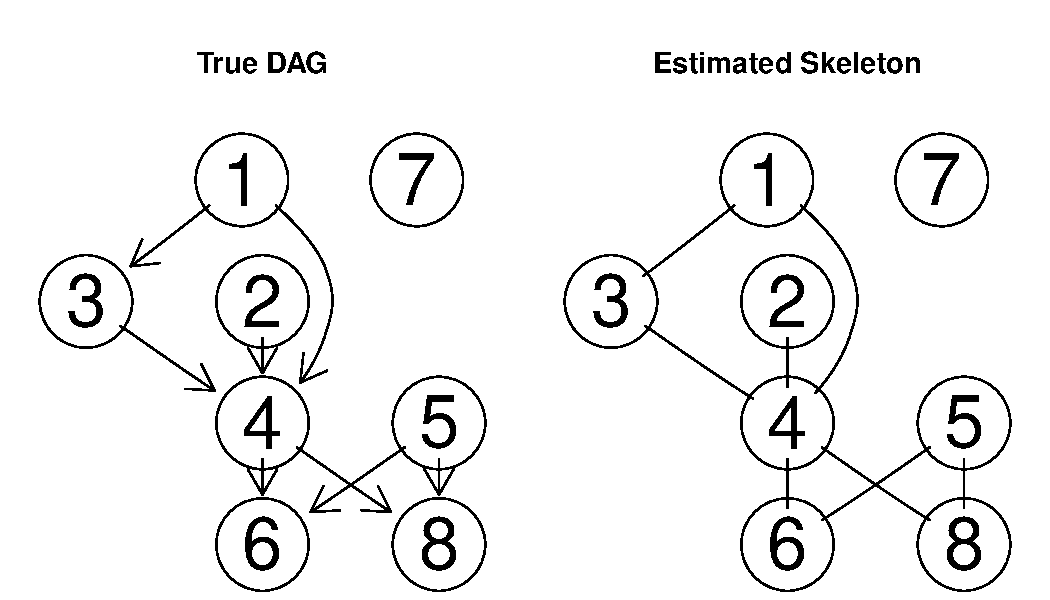
\includegraphics{pcalgDoc-skelExpl1Plot}
\caption{Estimated skeleton fitted on the gaussian data set provided by the
  package using the function \code{skeleton}.}
\label{fig:skelExpl}
\end{center}
\end{figure}

To give another example, we show how to fit a skeleton to the example data
set \code{discreteData} (which consists of $p=5$ discrete variables with 3,
2, 3, 4 and 2 levels and $n=10000$ samples). The predefined test function
\code{disCItest} is based on the $G^2$ statistics and takes as input a list
containing the data matrix, a vector specifying the number of levels for
each variable and and option which indicates whether to lower the degrees
of freedom by one for each zero count.

\begin{Schunk}
\begin{Sinput}
> ## load data matrix "dat"
> data(discreteData)
> p <- ncol(dat)
> ## use predefined test for discrete variables
> indepTest <- disCItest
> ## the function disCItest needs as input a list containing
> ## the data matrix, the number of levels for each variable and 
> ## a boolean variable indicating whether to adapt the degrees of freedom
> ## for zero counts
> suffStat <- list(dm = dat, nlev = c(3,2,3,4,2), adaptDF = FALSE)
> ## estimate skeleton 
> alpha <- 0.01 
> skel.fit <- skeleton(suffStat, indepTest, p, alpha)
> ## show estimated skeleton
> plot(skel.fit, main = "")
\end{Sinput}
\end{Schunk}
\begin{figure}
  \begin{center}
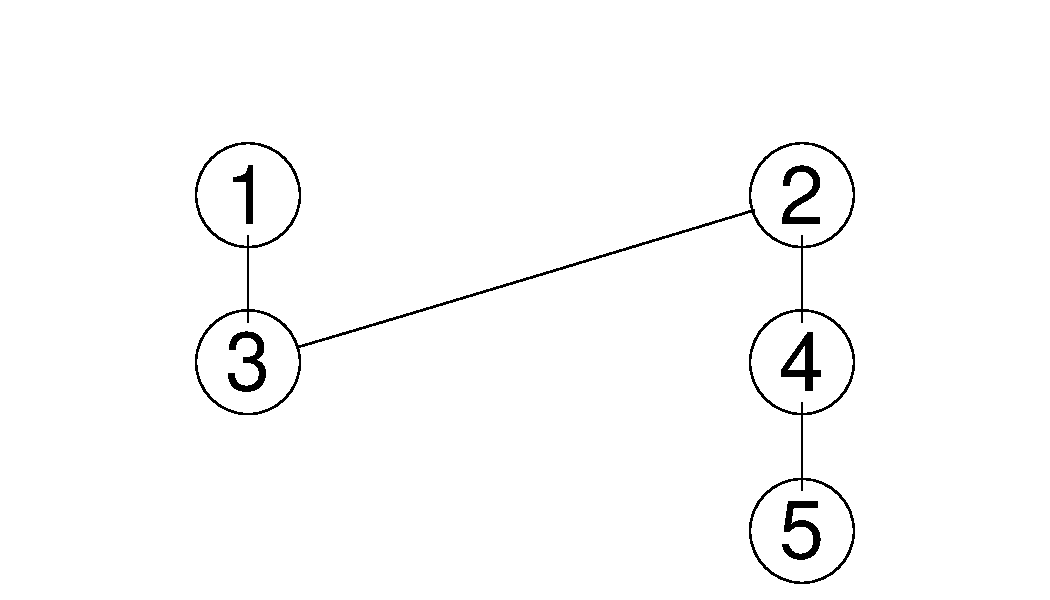
\includegraphics{pcalgDoc-skelExp2Plot}
\caption{Estimated skeleton fitted on the discrete data set provided by the
  package using the function \code{skeleton}.}
\label{fig:skel2}
\end{center}
\end{figure}

[XXX EXPLAIN STRUCTURE OF fixedGaps and fixedEdges: Bool AdjMatrix] The information in \texttt{fixedGaps} and \texttt{fixedEdges} is used as
follows.  The gaps given in \texttt{fixedGaps} are introduced in the very
beginning of the algorithm by removing the corresponding edges from the
complete undirected graph. Thus, these gaps are guaranteed to be in the
resulting graph. Pairs $(i,j)$ in \texttt{fixedEdges} are skipped in
all steps of the algorithm, so that these edges are guaranteed to be in the
resulting graph.

If \code{indepTest} returns \texttt{NA} and the option \code{NAdelete} is
\texttt{TRUE}, the corresponding edge is deleted. If this option is
\texttt{FALSE}, the edge is not deleted.

The argument \code{m.max} is the maximal size of the conditioning sets that
are considered in the conditional independence tests in (P2) of section \ref{sec:gm}.
          
Throughout, the function works with the column positions of the
variables in the adjacency matrix, and not with the names of the variables.

\subsection{pc} \label{sec:pc}
The function \code{pc} implements (P1) to (P4) of the PC
algorithm in two steps. First, the skeleton is computed using
the function \code{skeleton} and then as many edges as possible are
directed. The function can be called with the following arguments.

\code{pc(suffStat, indepTest, p, alpha, verbose = FALSE, fixedGaps = NULL,
fixedEdges = NULL, NAdelete = TRUE, m.max = Inf, u2pd = "rand")}
     
The options \code{suffStat, indepTest, p, alpha, fixedGaps,
  fixedEdges, NAdelete} and \code{m.max} are identical to those of the
function \code{skeleton}.

Sampling errors (or hidden variables) can lead to conflicting information
about edge directions. For example, one may find that $a-b-c$ and $b-c-d$
should both be directed as v-structures.  This gives conflicting
information about the edge $b-c$, since it should be directed as $b
\leftarrow c$ in v-structure $a \rightarrow b \leftarrow c$, while it
should be directed as $b \rightarrow c$ in v-structure $b \rightarrow c
\leftarrow d$. In such cases, we simply overwrite the directions of the
conflicting edge. In the example above this means that we obtain $a
\rightarrow b \rightarrow c \leftarrow d$ if $a-b-c$ was visited first, and
$a \rightarrow b \leftarrow c \leftarrow d$ if $b-c-d$ was visited first.

Sampling errors or hidden variables can also lead to invalid CPDAGs,
meaning that there does not exist a DAG that has the same skeleton and
v-structures as the graph found by the algorithm. An example of this is an
undirected cycle consisting of the edges $a-b-c-d$ and $d-a$. In this case it
is impossible to direct the edges without creating a cycle or a new
v-structure. The option \texttt{u2pd} specifies what should be done in such a
situation. If the option is set to \texttt{"relaxed"}, the algorithm simply
outputs the invalid CPDAG. If the option is set to \texttt{"rand"}, all direction
information is discarded and a random DAG is generated on the skeleton. If
the option is set to \texttt{"retry"}, up to 100 combinations of possible
directions of the ambiguous edges are tried, and the first combination that
results in a valid CPDAG is chosen. If no valid combination is found, an
arbitrary DAG is generated on the skeleton as in the option \texttt{"rand"}.

As with the skeleton, the algorithm works with the column positions of the
variables in the adjacency matrix, and not with the names of the
variables. When plotting the object, undirected and bidirected edges are
equivalent.


As an example, we estimate a CPDAG of the gaussian data used in the example
for the skeleton.

\begin{Schunk}
\begin{Sinput}
> ## load data matrix "dat"
> data(gaussianData)
> ## use predefined test for conditional independence on gaussian data
> indepTest <- gaussCItest 
> ## the functin gaussCItest needs as input a list with
> ## the correlation matrix C and the sample size n
> suffStat <- list(C = cor(dat), n = 5000)
> ## estimate the skeleton
> pc.fit <- pc(suffStat, indepTest, p = 8, alpha = 0.01)
> ## plot the resulting skeleton
> plot(pc.fit, main = "")
\end{Sinput}
\end{Schunk}
\begin{figure}
  \begin{center}
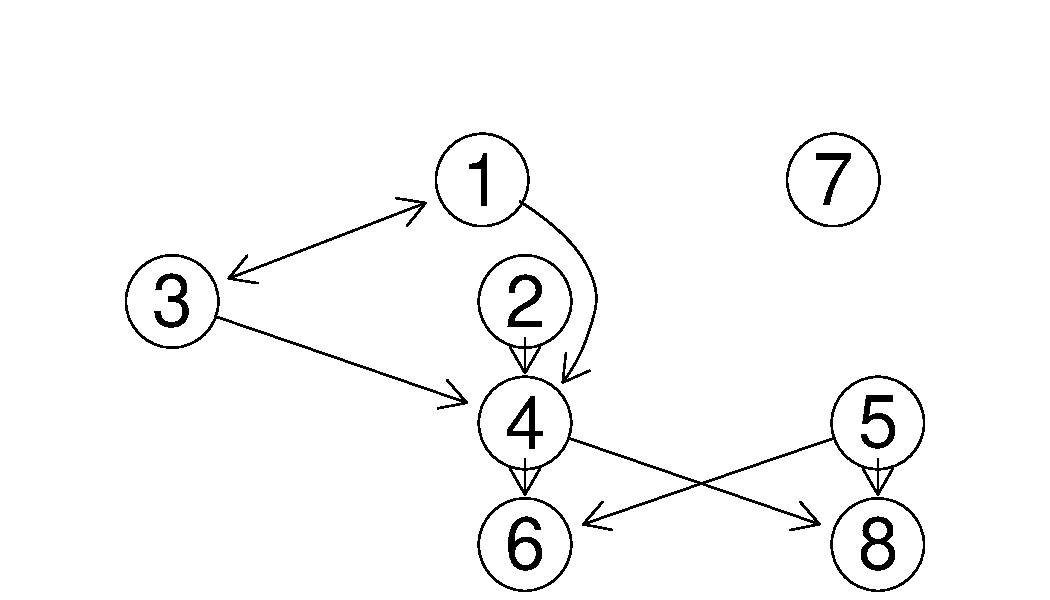
\includegraphics{pcalgDoc-011}
\caption{Estimated CPDAG fitted on the gaussian data set provided by the
  package using the function \code{pc}.}
\label{fig:pcFit1}
\end{center}
\end{figure}

\subsection{fci}
This function is a generalization of the PC algorithm (see section
\ref{sec:pc}), in the sense that it allows arbitrarily many latent and
selection variables. Under the assumption that the data are faithful to a
DAG that includes all latent and selection variables, the FCI algorithm
(Fast Causal Inference algorithm) estimates the equivalence class of MAGs
that describe the conditional independence relationships between the
observed variables.

We estimate an equivalence class of MAGs instead of DAGs, since DAGs are
not closed under marginalization and conditioning (Richardson and Spirtes,
2002). This means that if we start with a distribution that can be
represented by a DAG, it might be that the distribution we obtain by
marginalizing or conditioning out a variable is not representable by a
DAG. If we, however, use MAGs instead of DAGs, this cannot happen.

An equivalence class of a MAG can be uniquely represented by a partial
ancestral graph (PAG). A PAG contains the following types of edges: o-o,
o-, o->, ->, <->, -. The bidirected edges come from hidden variables, and
the undirected edges come from selection variables. The edges have the
following interpretation: (i) there is an edge between $x$ and $y$ if and
only if variables and are conditionally dependent given S for all sets S
consisting of all selection variables and a subset of the observed
variables; (ii) a tail on an edge means that this tail is present in all
MAGs in the equivalence class; (iii) an errowhead on an edge means that
this arrowhead is present in all MAGs in the equivalence class; (iv) a
o-edgemark means that there is a at least one MAG in the equivalence class
where the edgemark is a tail, and at least one where the edgemark is an
arrowhead. Information on the interpretation of edges in a MAG can be found
in the references given below.

The first part of the FCI algorithm is analogous to the PC algorithm. It
starts with a complete undirected graph and estimates an initial skeleton
using the function \code{skeleton}. All edges of this skeleton are of the
form o-o. Due to the presence of hidden variables, it is no longer
sufficient to consider only subsets of the neighborhoods of nodes $x$ and
$y$ to decide whether the edge $x-y$ should be removed.  Therefore, the
initial skeleton may contain some superfluous edges.  These edges are
removed in the next step of the algorithm. To decide whether edge $x o-o y$
should be removed, one computes Possible-D-SEP($x$) and Possible-D-SEP($y$)
and performs conditional indepedence tests of $x$ and $y$ given all
possible subsets of Possible-D-SEP($x$) and of Possible-D-SEP($y$) (see
helpfile of function \code{pdsep}). Subsequently, the v-structures are
determined (using information in sepset).  Finally, as many as possible
undetermined edge marks (o) are determined using (a subset of) the 10
orientation rules given by Zhang (2009).

\code{fci(suffStat, indepTest, p, alpha, verbose = FALSE, fixedGaps = NULL,\\
  fixedEdges = NULL, NAdelete = TRUE, m.max = Inf, rules = rep(TRUE, 10),\\
  doPdsep = TRUE)}
     
The options \code{suffStat, indepTest, p, alpha, fixedGaps, fixedEdges
,NAdelete} and \code{m.max} are identical to those in function
\code{skeleton}. The option \code{rules} contains a logical vector of
length 10 indicating which rules should be used when directing edges. The
order of the rules is taken from Zhang (2009).
     
The option \code{doPdsep} indicates, whether the Possible-D-SEP should be
computed. If TRUE, Possible-D-SEP is computed for all nodes, and all
subsets of Possible-D-SEP are considered as conditioning sets in the
conditional independence tests. If FALSE, Possible-D-SEP is not computed,
so that the algorithm simplifies to the Modified PC algorithm of Spirtes,
Glymour and Scheines (2000, page ...).
     
As an example, we estimate the PAG of a graph with five nodes one of which
is latent.
\begin{Schunk}
\begin{Sinput}
> ## data(latentVarGraph)
> load("/u/kalisch/research/packages/pcalg/data/latentVarGraph.rda")
> ## Information on node one is latent
> ## Data matrix "dat" contains data on remaining four nodes
> suffStat1 <- list(C = cor(dat), n = nrow(dat))
> indepTest1 <- gaussCItest 
> pag.est <- fci(suffStat1, indepTest1, ncol(dat), alpha = 0.01, verbose=FALSE)
\end{Sinput}
\end{Schunk}

\begin{figure}
  \begin{center}
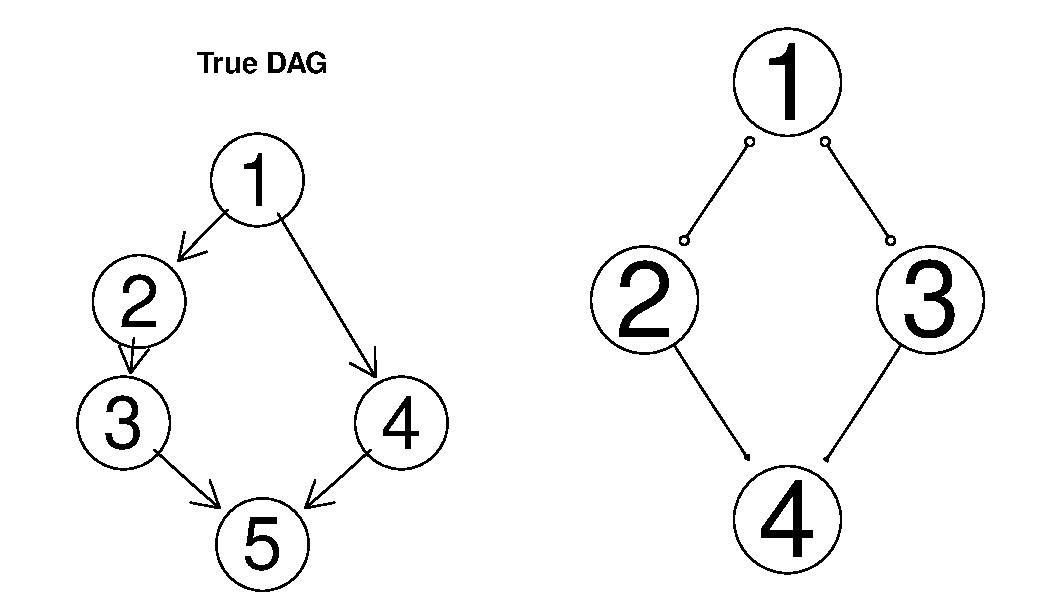
\includegraphics{pcalgDoc-013}
\caption{True data generating DAG and estimated PAG. Variable 1 of the data
generating DAG is latent. One can see, that the PAG was estimated correctly
(EXPLAIN MORE).}
\label{fig:fci}
\end{center}
\end{figure}

\subsection{ida} \label{sec:ida}
It is assumed that we have observational data that are multivariate
Gaussian and faithful to the true (but unknown) underlying causal DAG
(without hidden variables).  Under these assumptions, this function
estimates the multiset of possible total causal effects of $x$ on $y$,
where the total causal effect is defined via Pearl's do-calculus as
$E(Y|do(X=z+1))-E(Y|do(X=z))$ (this value does not depend on $z$, since
Gaussianity implies that conditional expectations are linear). We estimate
a set of possible total causal effects instead of the unique total causal
effect, since it is typically impossible to identify the latter when the
true underlying causal DAG is unknown (even with an infinite amount of
data).

To illustrate this, consider the following example. We have data from seven
gaussian variables with a causal structure given on the left of
Fig. \ref{fig:ida}. Denote node $i$ in the graph by $Vi$. We assume that
the causal structure is unknown and want to infer the causal effect of $V2$
on $V5$. First, we estimate the equivalence class of DAGs that describe the
conditional independence relationships in the data, using the function
\code{pc} (see section \ref{sec:pc}).

\begin{Schunk}
\begin{Sinput}
> ## load data matrix "dat"
> load("/u/kalisch/research/packages/pcalg/data/idaData.rda")
> ## data(idaData)
> 
> ## estimate CPDAG (see the help-file of the function "pc")
> indepTest <- gaussCItest 
> suffStat <- list(C = cor(dat), n = nrow(dat))
> pc.fit <- pc(suffStat, indepTest, p = ncol(dat), alpha = 0.01)
\end{Sinput}
\end{Schunk}

Comparing the true DAG with the CPDAG in Fig. \ref{fig:ida}, we see that
the CPDAG and the true DAG have the same skeleton. Moreover, the directed
edges in the CPDAG are also directed in that way in the true DAG. Three
edges in the CPDAG are bidirected. Recall that undirected and bidirected
edges bear the same meaning, so they can be used interchangeably.
\begin{figure}
  \begin{center}
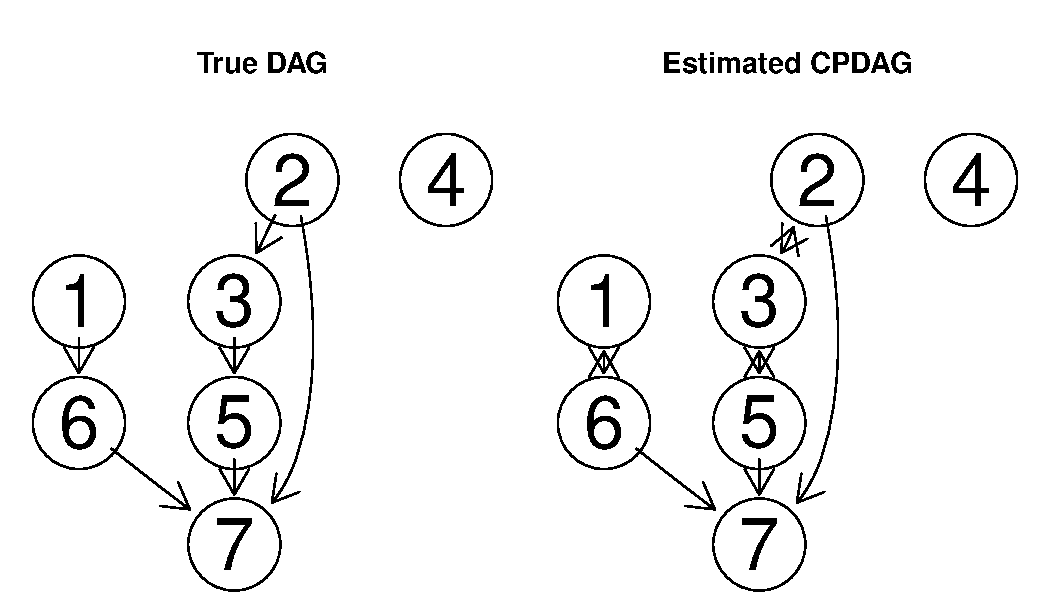
\includegraphics{pcalgDoc-idaExpl2}
\caption{True DAG and estimated CPDAG for illustrating the function \code{ida}}
\label{fig:ida}
\end{center}
\end{figure}

Since there are three undirected edges in the CPDAG, there might be up to
$2^3 = 8$ DAGs in the corresponding equivalence class. However, the
undirected edges $V2-V3-V5$ can be formed to a new v-structures. As
mentioned in section \ref{sec:gm}, DAGs in the equivalence class must have
exactly the same v-structures as the corresponding CPDAG. Thus, $V2-V3-V5$
can only be directed as $V2 \rightarrow V3 \rightarrow V5$, $V2 \leftarrow
V3 \leftarrow V5$ or $V2 \leftarrow V3 \rightarrow V5$ but not as $V2
\rightarrow V3 \leftarrow V5$, since tis would introduce a new colliding
v-structure. There is only one remaining undirected edge ($V1-V6$), which
can be directed in two ways. Thus, there are two out of the eight possible
DAGs that have a new v-structure and must therefore be excluded. The
remaining six DAGs are all valid (i.e. they have no new v-structure and no
cycle) and form the equivalence class represented by the CPDAG. In
Fig. \ref{fig:allDags}, all DAGs in the equivalence class are shown. DAG 4
is the true DAG. 

\begin{figure}
  \begin{center}
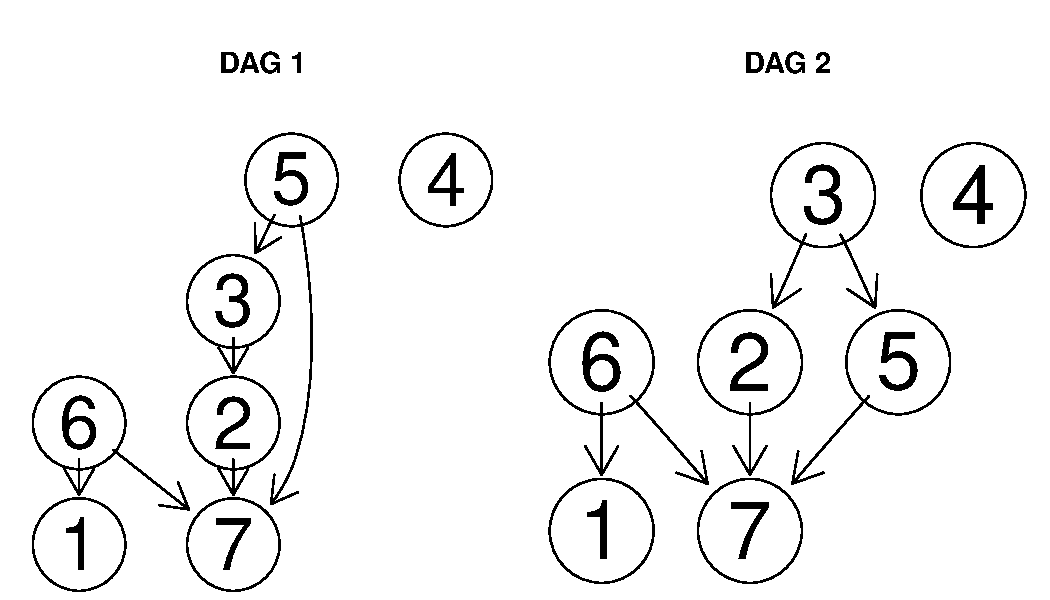
\includegraphics{pcalgDoc-017}
\caption{[XXX Einzelne plots; auf ganze Seite.] All DAGs belonging to the
  equivalence class represented by the CPDAG shown in Fig. \ref{fig:ida}}
\label{fig:allDags}
\end{center}
\end{figure}

For each DAG G in the equivalence class, we apply Pearl's do-calculus to
estimate the total causal effect of $x$ on $y$. This can be done via a
simple linear regression: if $y$ is not a parent of $x$, we take the
regression coefficient of $x$ in the regression \texttt{lm(y \~ x +
  pa(x))}, where \texttt{pa(x)} denotes the parents of $x$ in the DAG G; if
$y$ is a parent of $x$ in G, we set the estimated causal effect to zero.

If the equivalence class contains $k$ DAGs, this will yield $k$ estimated
total causal effects. Since we do not know which DAG is the true causal
DAG, we do not know which estimated total causal effect of $x$ on $y$ is
the correct one. Therefore, we return the entire multiset of $k$ estimated
effects (it is a multiset rather than a set because it can contain
duplicate values).

In our example, there are six DAGs in the equivalence class. Therefore, the
function \code{ida} will produce six possible values of causal effects (one
for each DAG). 

\begin{Schunk}
\begin{Sinput}
> ## Estimate the causal effect of 2 on 5
> ## True Effekt of 2 on 5: 0.5529
>      ida(2, 5, cov(dat), pc.fit@graph, method = "global", verbose = FALSE)
\end{Sinput}
\begin{Soutput}
[1] -0.004901204 -0.004901204  0.542135970 -0.004901204 -0.004901204
[6]  0.542135970
\end{Soutput}
\end{Schunk}

Among these six values, there are only two unique values: $-0.0049$ and
$0.5421$. This is because we compute \texttt{lm(V5 ~ V2 + pa(V2))} ($Vi$
denotes node $i$) for each
DAG and report the regression coefficient of $V2$. Note that there are
only two possible parent sets of $V2$ in all six DAGs: In DAGs 3 and 6,
there are no parents of $V5$. In DAGs 1, 2, 4 and 5, however, the parent
of $V2$ is $V3$. Thus, exactly the same regressions are computed for
DAGs 3 and 6 and the same regressions are computed for DAGs 1, 2, 4 and 5.

Since the data was simulated from a model, we know that the true value the
causal effect of $V2$ on $V5$ is $0.5529$. Thus, one of the two unique values is
indeed very close to the true causal effect (the slight discrepancy is due
to sampling error). 

The function \code{ida} can be called with the following arguments.

\code{ida(x.pos, y.pos, mcov, graphEst, method = "local", y.notparent = FALSE,\\ 
verbose = FALSE, all.dags = NA)}

\texttt{x.pos} denotes the column position of the cause variable and
\texttt{y.pos} denotes the column position of the effect
variable. \texttt{mcov} is the covariance matrix of the original
data. \texttt{graphEst} is a graph object describing the causal structure
(this could be given by experts or estimated using the function \code{pc}).

If \texttt{method="global"}, the method as described above is carried out,
where all DAGs in the equivalene class of the estimated CPDAG are
computed. This method is suitable for small graphs (say, up to 10
nodes). The DAGs can (but need not) be precomputed using the function
\code{allDags} and passed via the option \texttt{all.dags}.

If \texttt{method="local"}, we do not determine all DAGs in the equivalence
class of the CPDAG. Instead, we only consider the local neighborhood of $x$
in the CPDAG. In particular, we consider all possible directions of
undirected edges that have $x$ as endpoint, such that no new v-structure is
created. For each such configuration, we estimate the total causal effect
of $x$ on $y$ as above, using linear regression.

At first sight, it is not clear that such a local configuration corresponds
to a DAG in the equivalence class of the CPDAG, since it may be impossible
to direct the remaining undirected edges without creating a directed cycle
or a v-structure. However, Maathuis, Kalisch and B\"uhlmann (2009) showed
that there is at least one DAG in the equivalence class for each such local
configuration.  As a result, it follows that the multisets of total causal
effects of the \texttt{global} and the \texttt{local} method have the same unique
values. They may, however, have different multiplicities. 

Recall, that in the example using the global method, we obtained as a
result two unique values with multiplicities two and four yielding six
numbers in total.  Applying the local method, we obtain the same unique
values, but the multiplicities are 1 for both values (they need not always
be one) and are thus different from the global method.
\begin{Schunk}
\begin{Sinput}
> ## Estimate the causal effect of 2 on 5
> ## True Effekt of 2 on 5: 0.5529
> ida(2,5,cov(dat),pc.fit@graph,method = "local")
\end{Sinput}
\begin{Soutput}
[1]  0.542135970 -0.004901204
\end{Soutput}
\end{Schunk}

One can take summary measures of the multiset. For example, the minimum
absolute value provides a lower bound on the size of the true causal
effect: if the minimum absolute value of all values in the multiset is
larger than one, then we know that the size of the absolute true causal
effect (up to sampling error) must be larger than one. The fact that the
unique values of the multisets of the \texttt{global} and \texttt{local}
method are identical implies that summary measures of the multiset that
only depend on the unique values (such as the minimum absolute value) can
be estimated by the local method.

In some applications, it is clear that some variable is definitively not an
effect but it migth be a cause. Consider for example a bacterium producing
a certain substance, taking the amount of produced substance as goal
variable. Knocking out genes in the bacterium might change the ability to
produce the substance. By measuring the expressin levels of genes, we want
to know which genes have a causal effect on the product. In this setting,
it is clear that the amount of substance is the effect and the activity of
the genes is the cause. Thus in the causal structure, the goal variable can
not be a parent node of any variable describing the expression level of
genes. This background knowledge can be easily incorporated: By setting the
option \texttt{y.notparent = TRUE}, all edges in the CPDAG connected to the
goal variable (no matter whether directed or undirected) are directed
towards the goal variable.

\subsection{idaFast}
In some applications it is desirable to estimate the causal effect of one
variable on a set of goal variables. In these situations, the function
\code{idaFast} should be used. Imagine for example, that we have data
on several variables and we have no background knowledge about the causal
effects among the variables. Thus, we want to estimate the causal effect of
each variable onto each other variable. To this end, we could consider for
each variable the problem: What is the causal effect of this variable on
all other variables. Of course, one could solve the problem by using \code{ida} on
each pair of variables. However, there is a more efficient way which uses
the fact, that a linear regression of a fixed set of explanatory variables
on several different goal variables can be computed very efficiently.

The function \code{idaFast} can be called with the following arguments.
\code{idaFast(x.pos, y.pos.set, mcov, graphEst)}
\texttt{x.pos}, \texttt{mcov}, \texttt{graphEst} have the same meaning as
the corresponding arguments in \code{ida}. \texttt{y.pos.set} is a vector
containg the column positions of all effect variables of interest.

This call performs \code{ida(x.pos, y.pos, mcov, graphEst, method="local",
  y.notparent=FALSE, verbose=FALSE)} for all values of \texttt{y.pos} in
\texttt{y.pos.set} at the same time and in an efficient way. Note that the
option \texttt{y.notparent = TRUE} is not implemented, since it is not
clear how to do that efficiently without orienting all edges away from
\texttt{y.pos.set} at the same time, which seems not to be desirable.

Consider the example from section \ref{sec:ida}, where we computed the
causal effect of $V2$ on $V5$. Now, we want to compute the effect of
$V2$ on $V5$, $V6$ and $V7$ using \code{idaFast}.
\begin{Schunk}
\begin{Sinput}
> ## Simulate the true DAG
> set.seed(123)
> p <- 7
> myDAG <- randomDAG(p, prob = 0.2) ## true DAG
> myCPDAG <- dag2cpdag(myDAG) ## true CPDAG
> covTrue <- trueCov(myDAG) ## true covariance matrix
> ## simulate data from the true DAG
> n <- 10000
> dat <- rmvDAG(n, myDAG)
> ## estimate CPDAG (see help on the function "pc")
> alpha <- 0.01
> indepTest <- gaussCItest 
> suffStat <- list(C = cor(dat), n = n)
> pc.fit <- pc(suffStat, indepTest, p, alpha)
> (eff.est1 <- ida(2,5,cov(dat),pc.fit@graph,method="local",verbose=FALSE))
\end{Sinput}
\begin{Soutput}
[1]  0.542135970 -0.004901204
\end{Soutput}
\begin{Sinput}
> (eff.est2 <- ida(2,6,cov(dat),pc.fit@graph,method="local",verbose=FALSE))
\end{Sinput}
\begin{Soutput}
[1] -0.005853153 -0.006231005
\end{Soutput}
\begin{Sinput}
> (eff.est3 <- ida(2,7,cov(dat),pc.fit@graph,method="local",verbose=FALSE))
\end{Sinput}
\begin{Soutput}
[1] 1.0086138 0.8970766
\end{Soutput}
\begin{Sinput}
> ## These three computations can be combinded in an efficient way by using idaFast
> (eff.estF <- idaFast(2,c(5,6,7),cov(dat),pc.fit@graph))
\end{Sinput}
\begin{Soutput}
      beta.tmp     beta.tmp
5  0.542135970 -0.004901204
6 -0.005853153 -0.006231005
7  1.008613785  0.897076593
\end{Soutput}
\end{Schunk}

\subsection{Using a user specific conditional independence test}
In some cases it might be desirable to use a user specific conditional
independence test instead of the provided ones. The \pkg{pcalg} package is
flexible enough to allow the use of any conditional independence test
defined by the user. In this section, we illustrate this feature by using a
conditional independence test for gaussian data that is not predefined in
the package.

The functions \code{skeleton}, \code{pc} and \code{fci} need for the
conditional independence tests a function of the form \code{myCItest(x, y, S,
  suffStat)}. This function must return the p-value of the conditional
indepence test of $x$ and $y$ given $S$ given some information on the data
in form of a sufficient statistic (this might be simply the data frame with
the original data). $x$, $y$, $S$ indicate column positions of the original
data matrix. We will show an example, of how to construct such a function. 

A simple way to compute the partial correlation of $x$ and $y$ given $S$
for some data is to solve the two associated linear regression problems $x
\sim S$ and $y \sim S$, get the residuals, and calculate the correlation
between the residuals. Finally, a correlation test between the residuals
yields a p-value that can be returned. The argument \texttt{suffStat} is an
arbitrary object containing several pieces of information that are all used
within the function to produce the p-value. In the predefined function
\code{gaussCItest} for example, a list containing the correlation matrix
and the number of observations is passed. This has the advantage, that any
favorite (e.g. robust) method of computing the correlation matrix can be
used before partial correlations are computed. Oftentimes, however, it will
suffice to just pass the complete data set in \texttt{suffStat}. We will
choose this simple way in our example. An implementation of the function
\code{myCItest} could look like this.
\begin{Schunk}
\begin{Sinput}
> myCItest <- function(x,y,S, suffStat) {
+   if (length(S) == 0) {
+     ## marginal case
+     res <- cor.test(suffStat[,x],suffStat[,y])$p.value
+   } else {
+     ## conditional case
+     resx <- resid(lm(suffStat[,x] ~ suffStat[,S]))
+     resy <- resid(lm(suffStat[,y] ~ suffStat[,S]))
+     res <- cor.test(resx, resy)$p.value
+   }
+   res
+ }
\end{Sinput}
\end{Schunk}
We can now use this function together with the \code{pc} function.

\begin{Schunk}
\begin{Sinput}
> data(gaussianData) ## contains data matrix dat
> indepTest <- myCItest 
> suffStat <- dat
> pc.myfit <- pc(suffStat, indepTest, p = 8, alpha = 0.01)
> ## plot the resulting causal structure
> par(mfrow = c(1,2))
> ## result using gaussCItest
> plot(pc.fit, main = "gaussCItest")
> plot(pc.myfit, main = "myCItest")
\end{Sinput}
\end{Schunk}

\begin{figure}
  \begin{center}
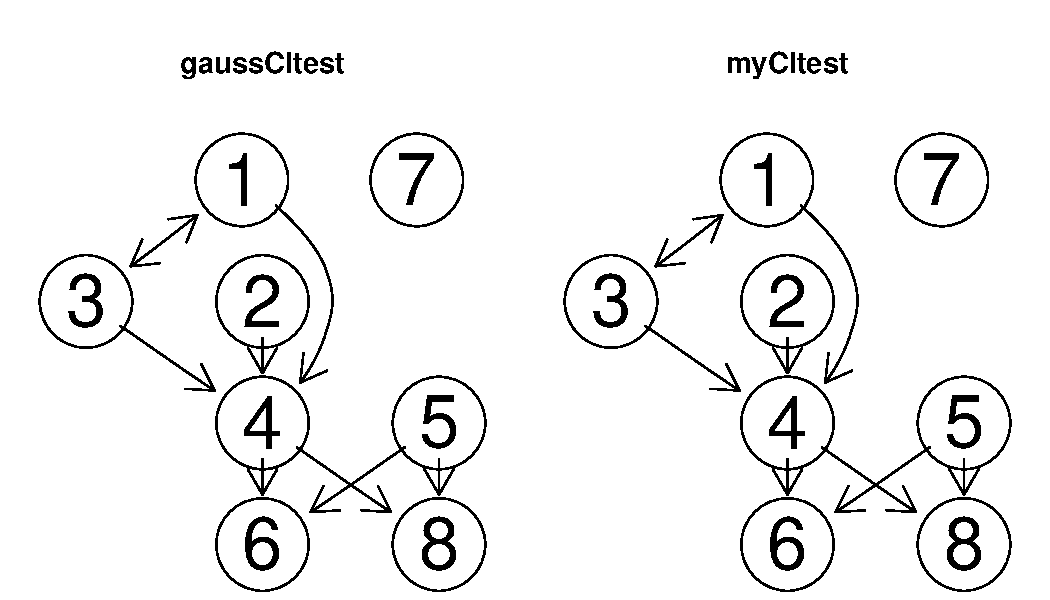
\includegraphics{pcalgDoc-024}
\caption{The estimated CPDAGs using the predefined and the user specified
  conditional independence test are identical.}
\label{fig:userSpec}
\end{center}
\end{figure}
As expected, the resulting CPDAG (see Fig. \ref{fig:userSpec}) is the same
as in section \ref{sec:pc} where we used the function \code{gaussCItest} as
conditional independence test. Note, however, that using
\code{gaussCItest} is considerably faster than using \code{myCItest} (on
our computer $0.067$ seconds using \code{gaussCItest} versus $4.448$
seconds using \code{myCItest}).

MENTION: S4-class gAlgo, pcAlgo, fciAlgo and inheritance.
\section{Conclusion}

\end{document}
